\subsubsection{UAP ResNet50}
\todo{Kapitel noch in Arbeit}
In diesem Kapitel visualisieren wir die UAP, welches durch das ResNet18 Modell erstellt wurden.

% UAPs Resnet18 covidx robustifikations level 0
\begin{figure}[ht!]
    \centering
    \begin{subfigure}{0.19\linewidth}
        \centering
        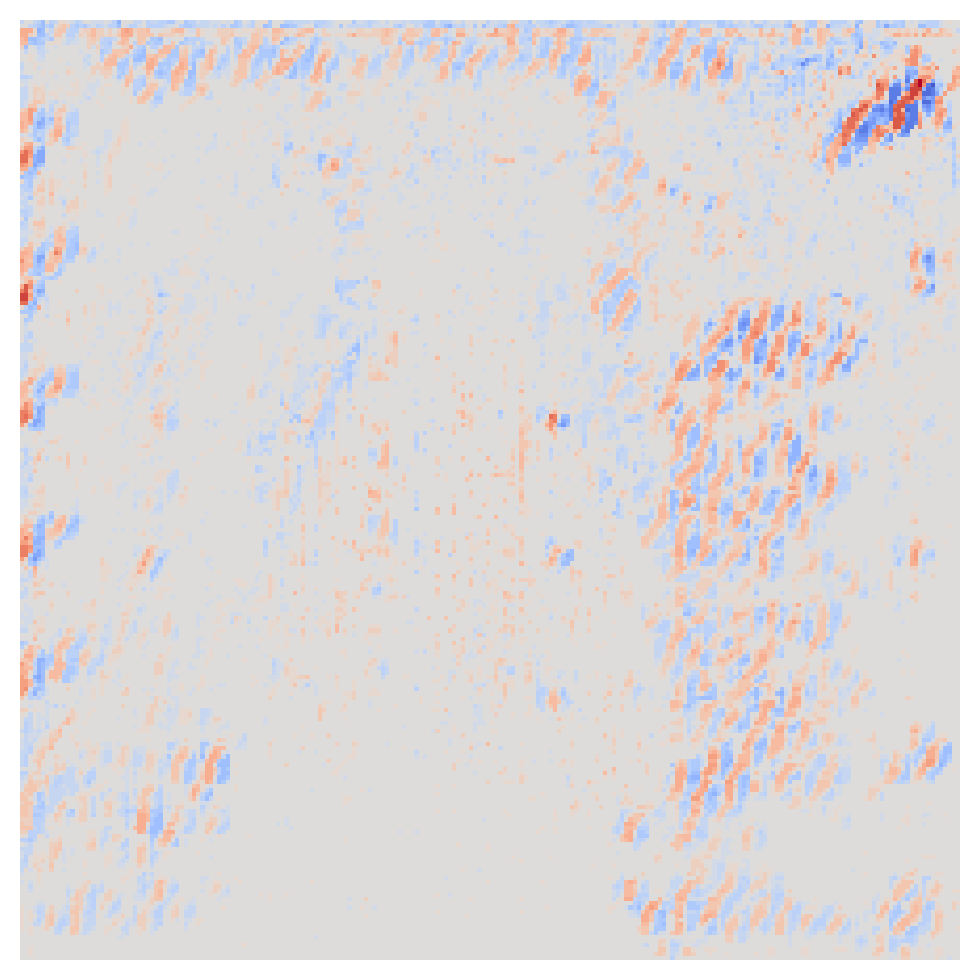
\includegraphics[height=1\linewidth]{01-images/05-resultate/uap_resnet/uap0-resnet18-covid-n200-robustificationslevel0.png}
        \caption{UAP Index 0}
    \end{subfigure}\hfill%
    \begin{subfigure}{0.19\linewidth}
        \centering
        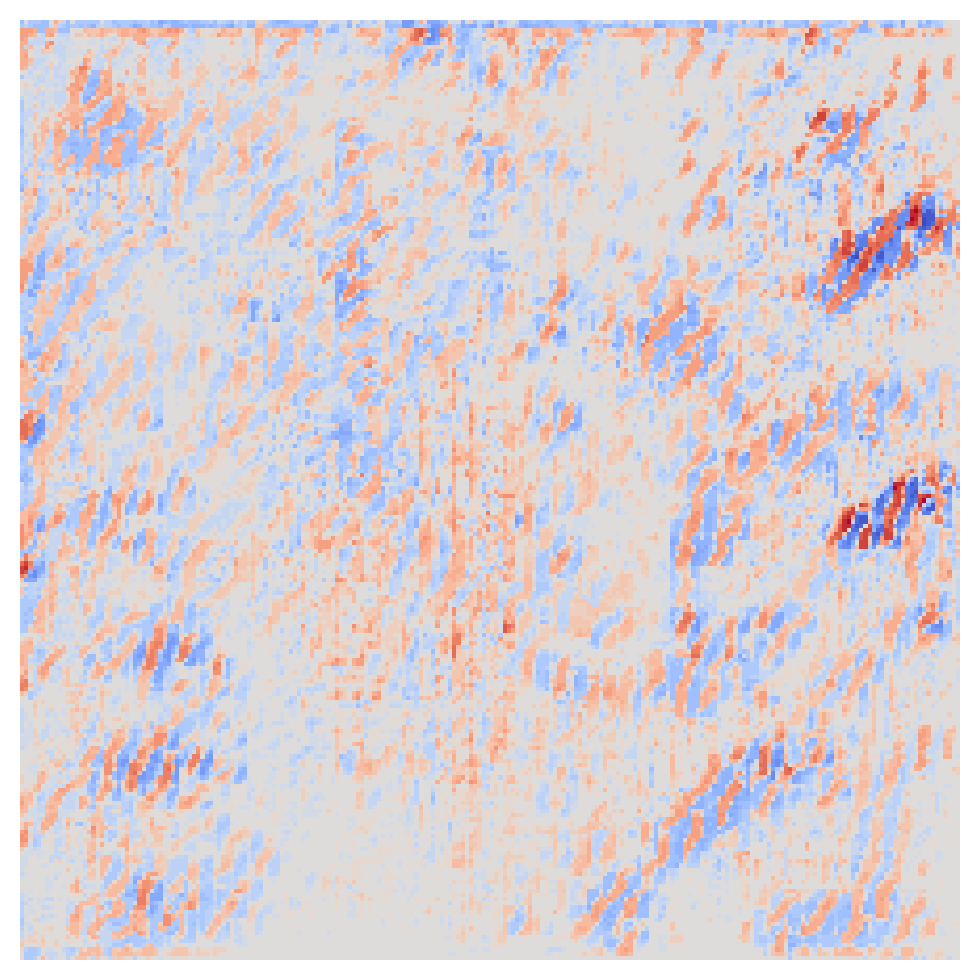
\includegraphics[height=1\linewidth]{01-images/05-resultate/uap_resnet/uap1-resnet18-covid-n200-robustificationslevel0.png}
        \caption{UAP Index 1}
    \end{subfigure}\hfill%
    \begin{subfigure}{0.19\linewidth}
        \centering
        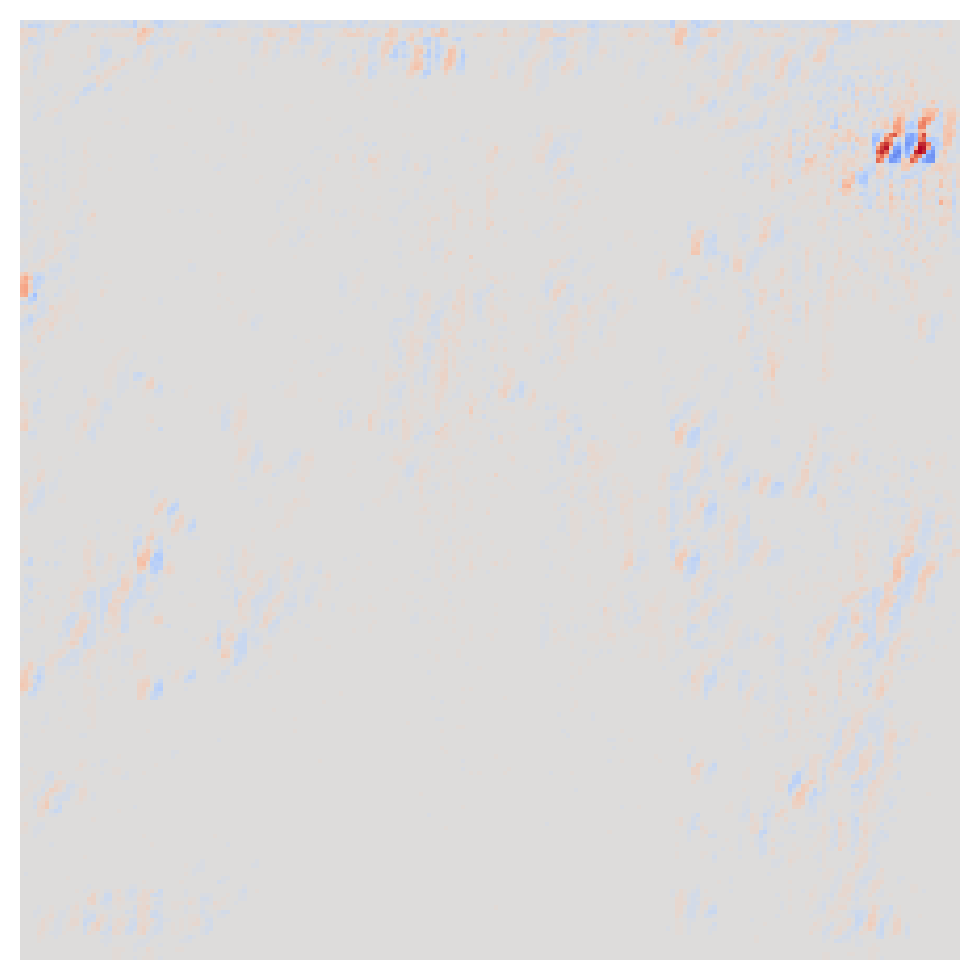
\includegraphics[height=1\linewidth]{01-images/05-resultate/uap_resnet/uap2-resnet18-covid-n200-robustificationslevel0.png}
        \caption{UAP Index 2}
    \end{subfigure}\hfill%
    \begin{subfigure}{0.19\linewidth}
        \centering
        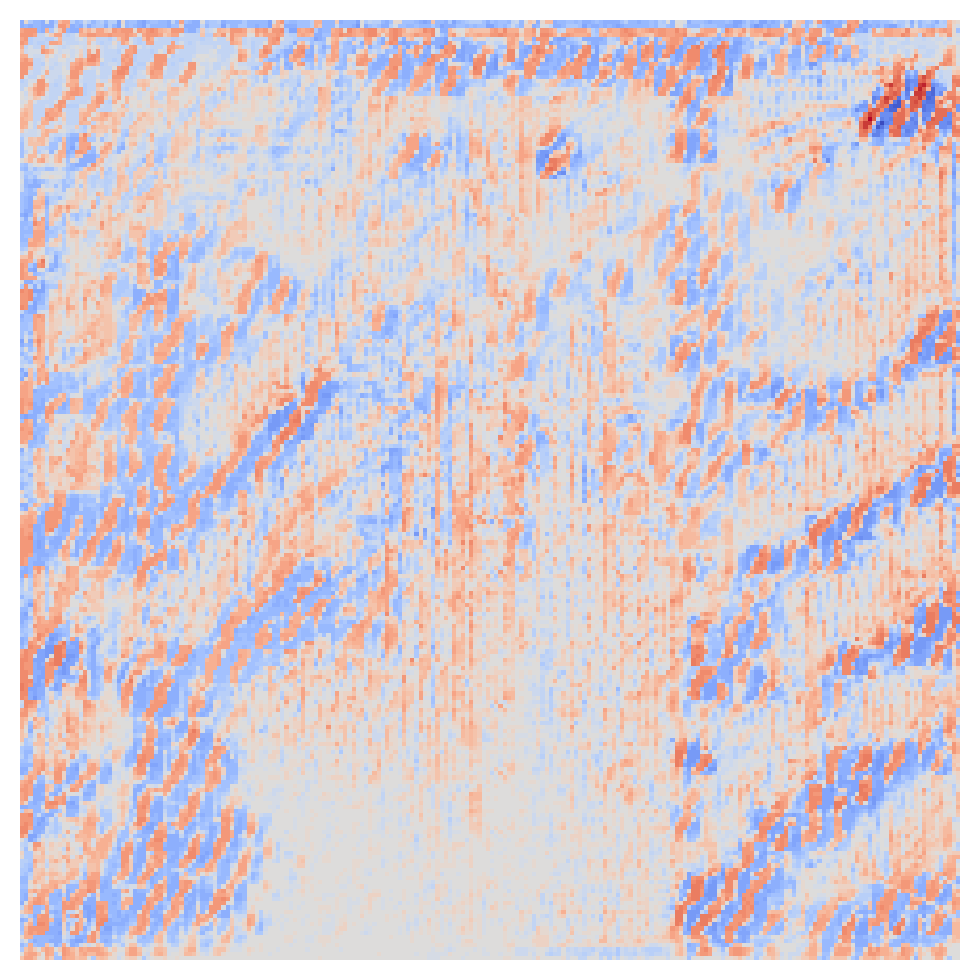
\includegraphics[height=1\linewidth]{01-images/05-resultate/uap_resnet/uap3-resnet18-covid-n200-robustificationslevel0.png}
        \caption{UAP Index 3}
    \end{subfigure}\hfill%
    \begin{subfigure}{0.19\linewidth}
        \centering
        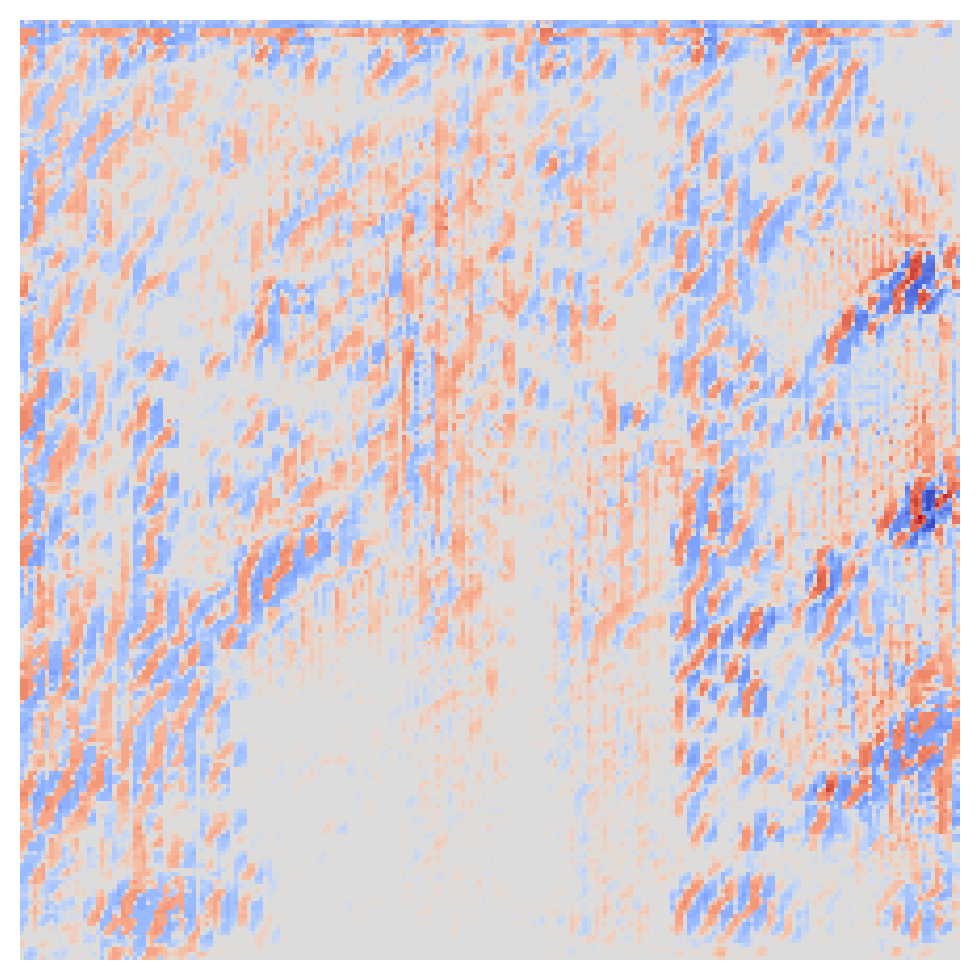
\includegraphics[height=1\linewidth]{01-images/05-resultate/uap_resnet/uap4-resnet18-covid-n200-robustificationslevel0.png}
        \caption{UAP Index 4}
    \end{subfigure}
    \caption{5 generierte UAPs durch 200 Trainingsbilder des mit ResNet18 trainierten Covidx Datensatzes vor der Robustifizierung durch adversarielles Training}
    \label{fig:uap-resnet18-covidx-rob0}
\end{figure}

in Abbildung \ref{} sind 5 UAPs vor der Robustifikation auf den Covidx Datensatz zu erkennen. 

% UAPs Resnet18 MRI robustifikations level 0
\begin{figure}[ht!]
    \centering
    \begin{subfigure}{0.19\linewidth}
        \centering
        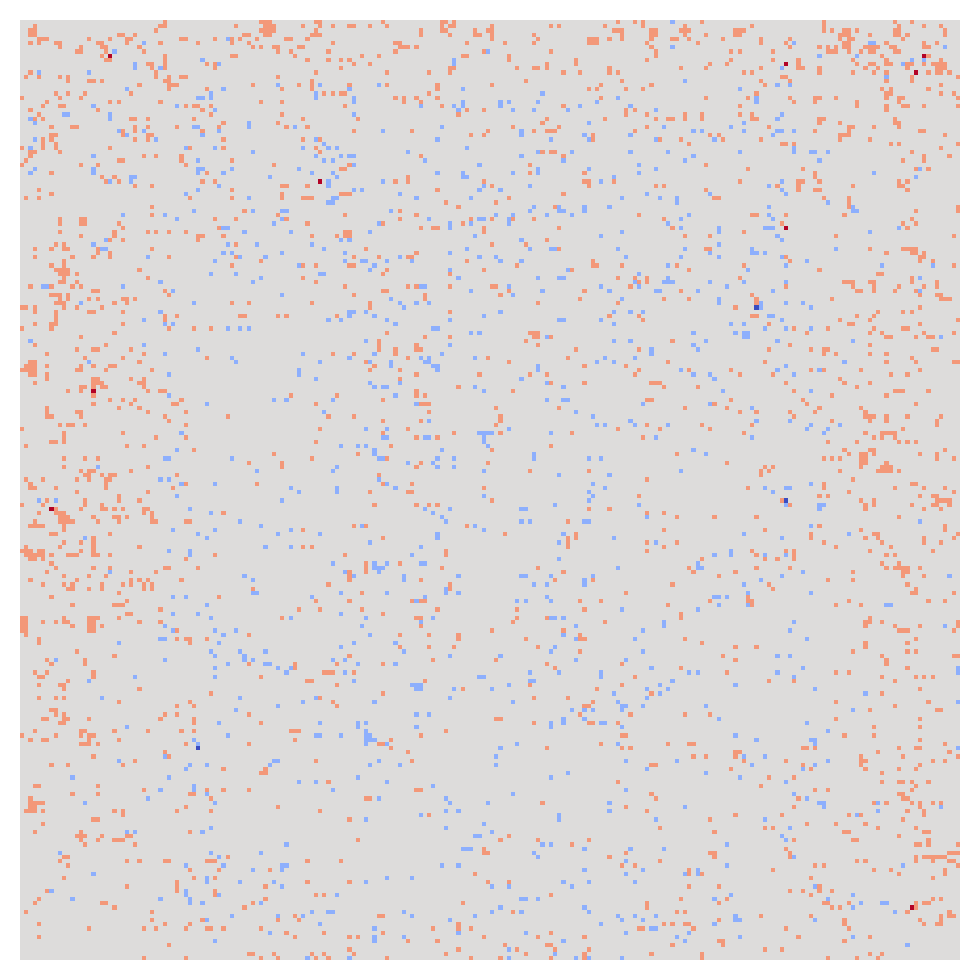
\includegraphics[height=1\linewidth]{01-images/05-resultate/uap_resnet/uap0-resnet18-mri-n200-robustificationslevel0.png}
        \caption{UAP Index 0}
    \end{subfigure}\hfill%
    \begin{subfigure}{0.19\linewidth}
        \centering
        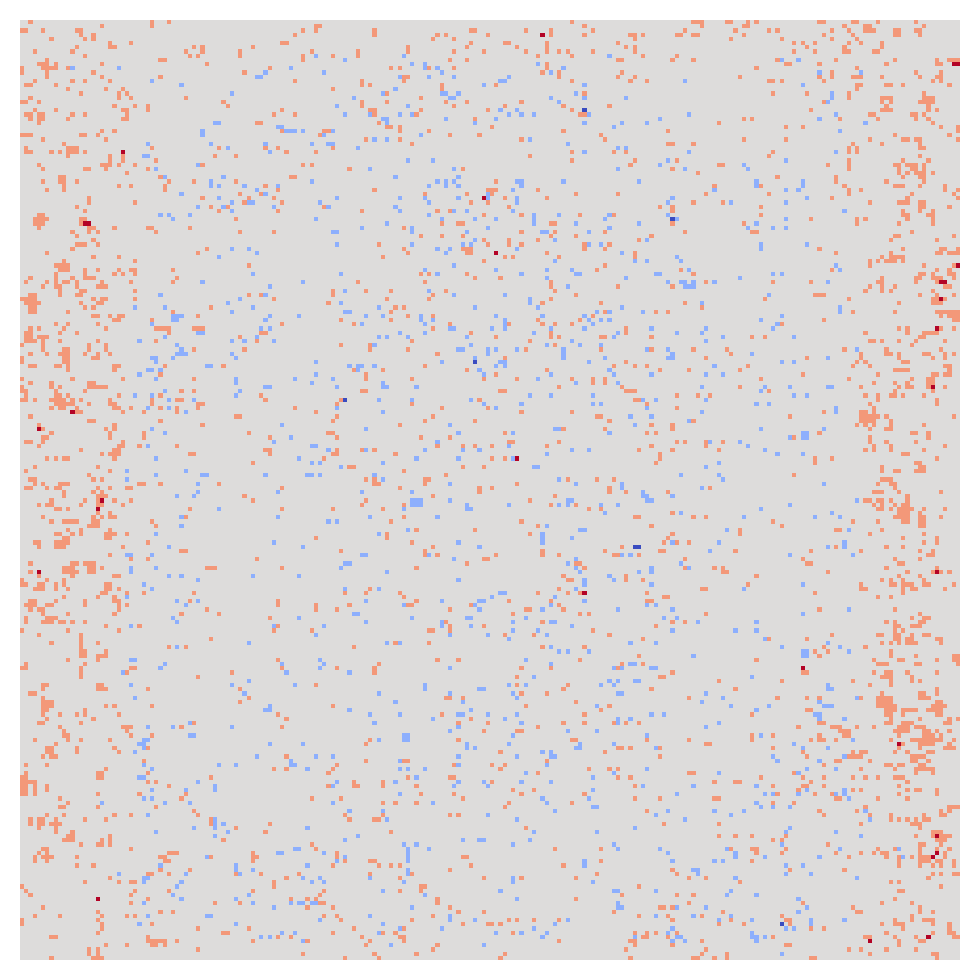
\includegraphics[height=1\linewidth]{01-images/05-resultate/uap_resnet/uap1-resnet18-mri-n200-robustificationslevel0.png}
        \caption{UAP Index 1}
    \end{subfigure}\hfill%
    \begin{subfigure}{0.19\linewidth}
        \centering
        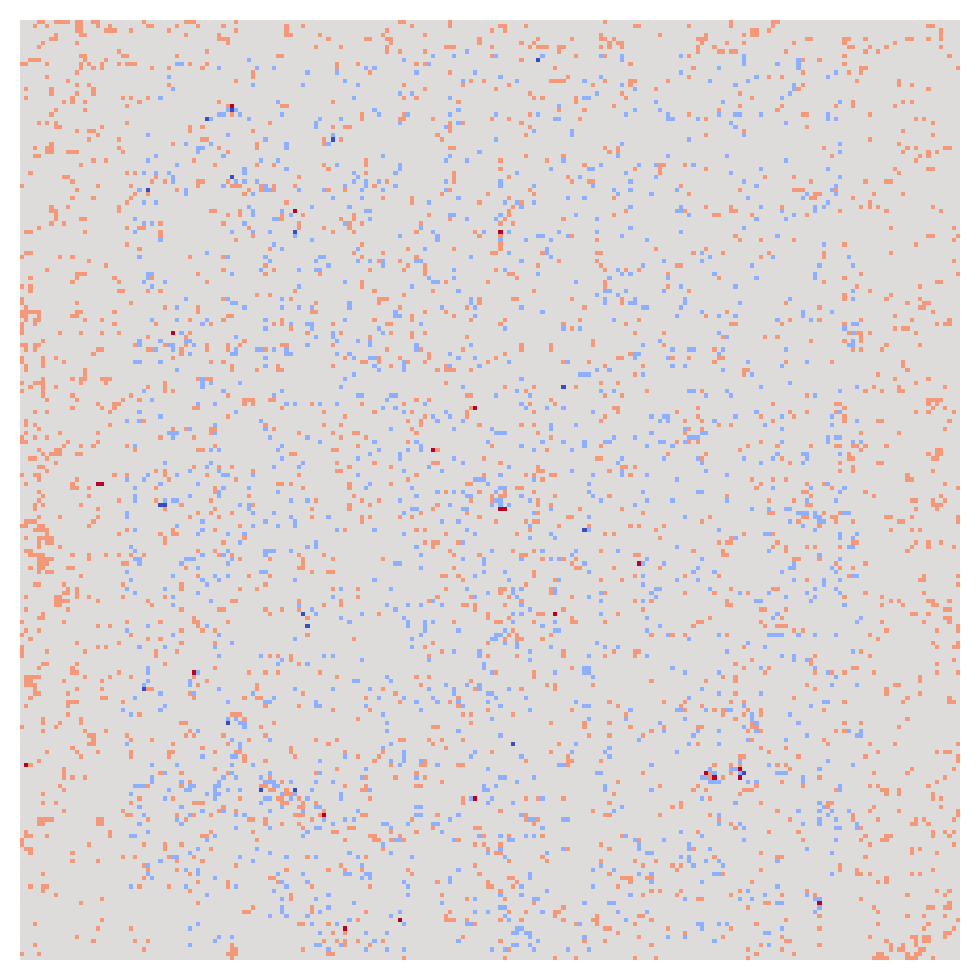
\includegraphics[height=1\linewidth]{01-images/05-resultate/uap_resnet/uap2-resnet18-mri-n200-robustificationslevel0.png}
        \caption{UAP Index 2}
    \end{subfigure}\hfill%
    \begin{subfigure}{0.19\linewidth}
        \centering
        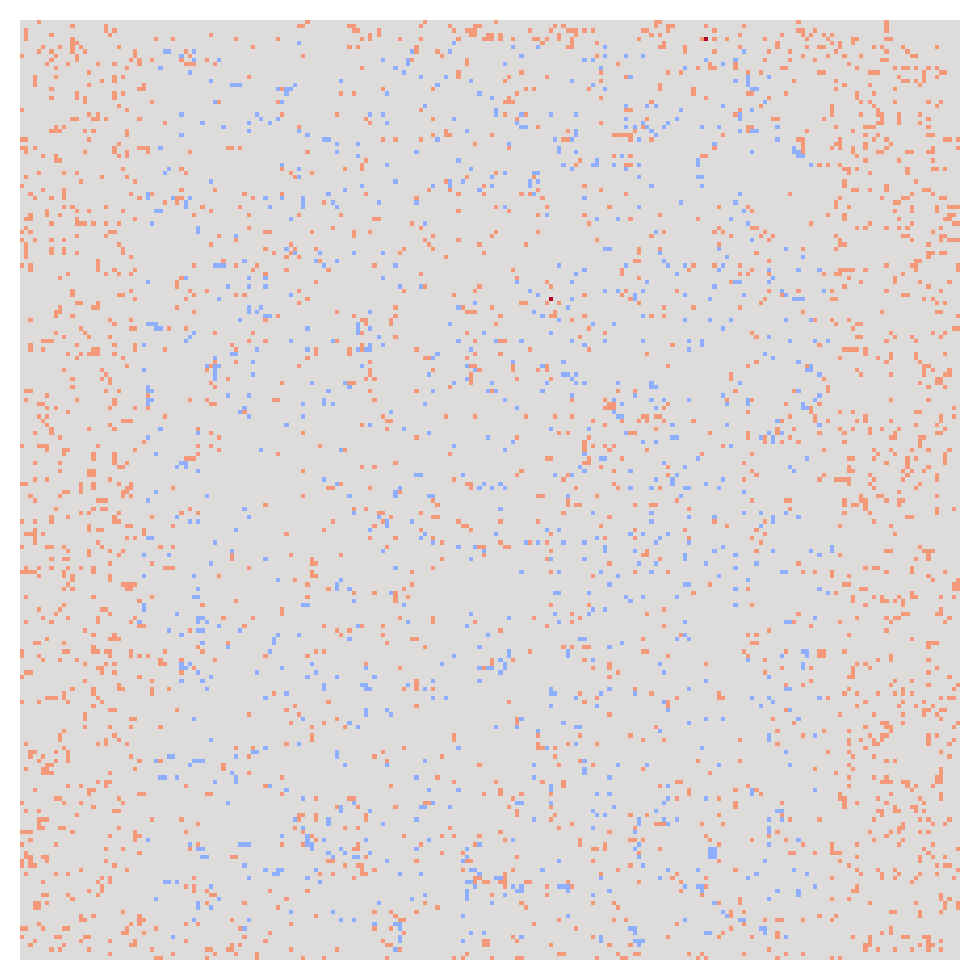
\includegraphics[height=1\linewidth]{01-images/05-resultate/uap_resnet/uap3-resnet18-mri-n200-robustificationslevel0.png}
        \caption{UAP Index 3}
    \end{subfigure}\hfill%
    \begin{subfigure}{0.19\linewidth}
        \centering
        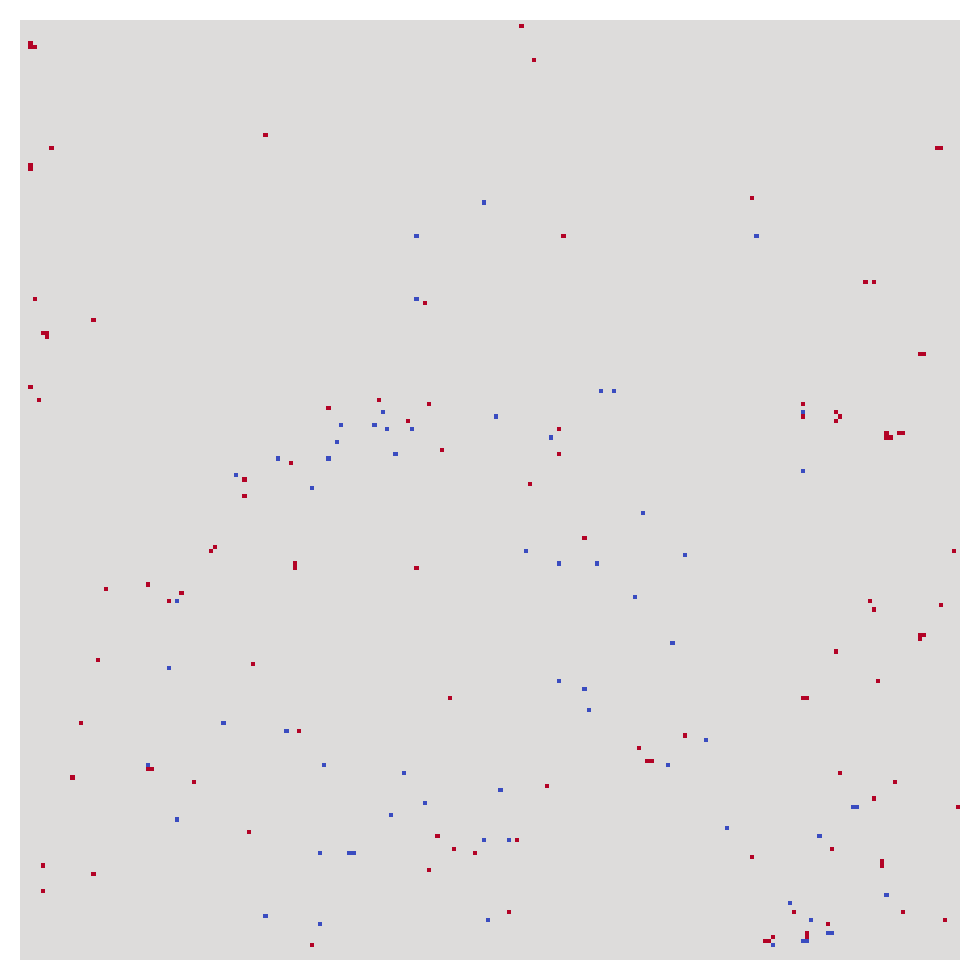
\includegraphics[height=1\linewidth]{01-images/05-resultate/uap_resnet/uap4-resnet18-mri-n200-robustificationslevel0.png}
        \caption{UAP Index 4}
    \end{subfigure}
    \caption{5 generierte UAPs durch 200 Trainingsbilder des mit ResNet18 trainierten Hirntumor Datensatzes vor der Robustifizierung durch adversarielles Training}
    \label{fig:uap-resnet18-mri-rob0}
\end{figure}

in Abbildung \ref{} sind 5 UAPs vor der Robustifikation auf den Hinrtumor Datensatz zu erkennen. 

\newpage

% UAP Vor und Nach Robustifikation
\begin{figure}[ht!]
    \centering
    \begin{subfigure}{0.19\linewidth}
        \centering
        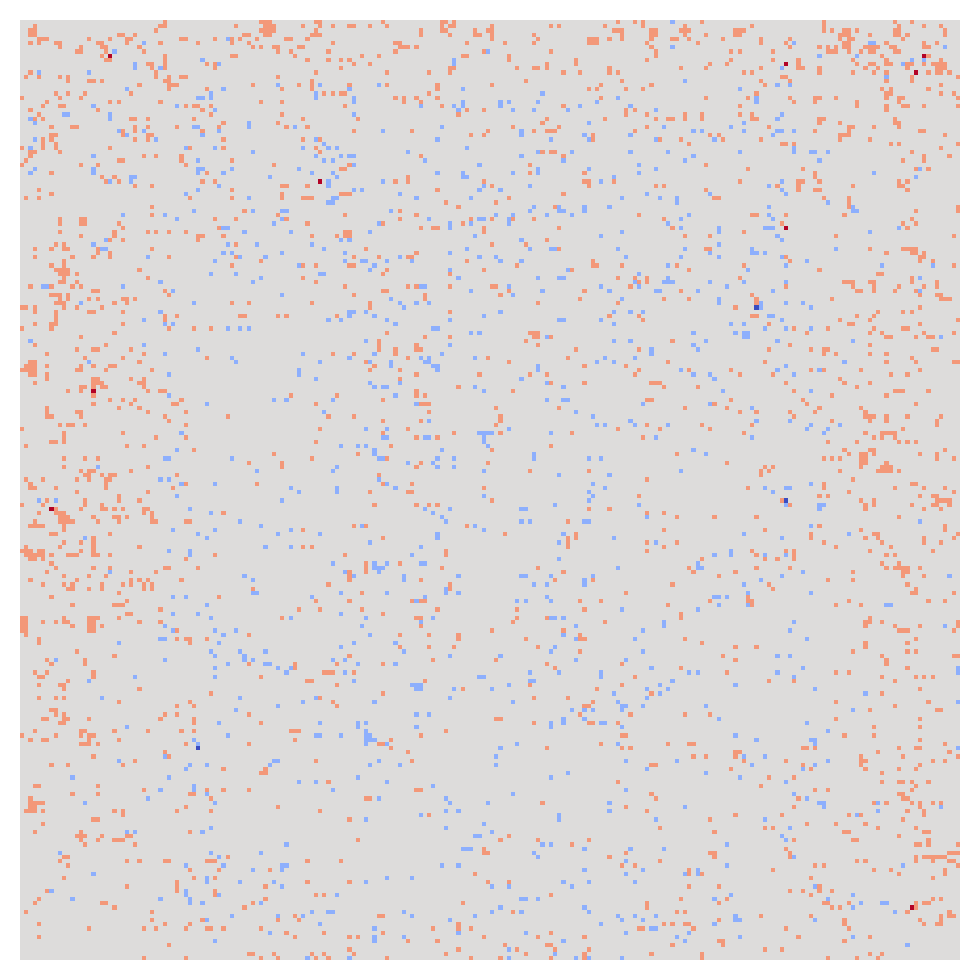
\includegraphics[height=1\linewidth]{01-images/05-resultate/uap_resnet/uap0-resnet18-mri-n200-robustificationslevel0.png}
        \caption{UAP 1 vor der Robustifikation}
    \end{subfigure}
    \begin{subfigure}{0.19\linewidth}
        \centering
        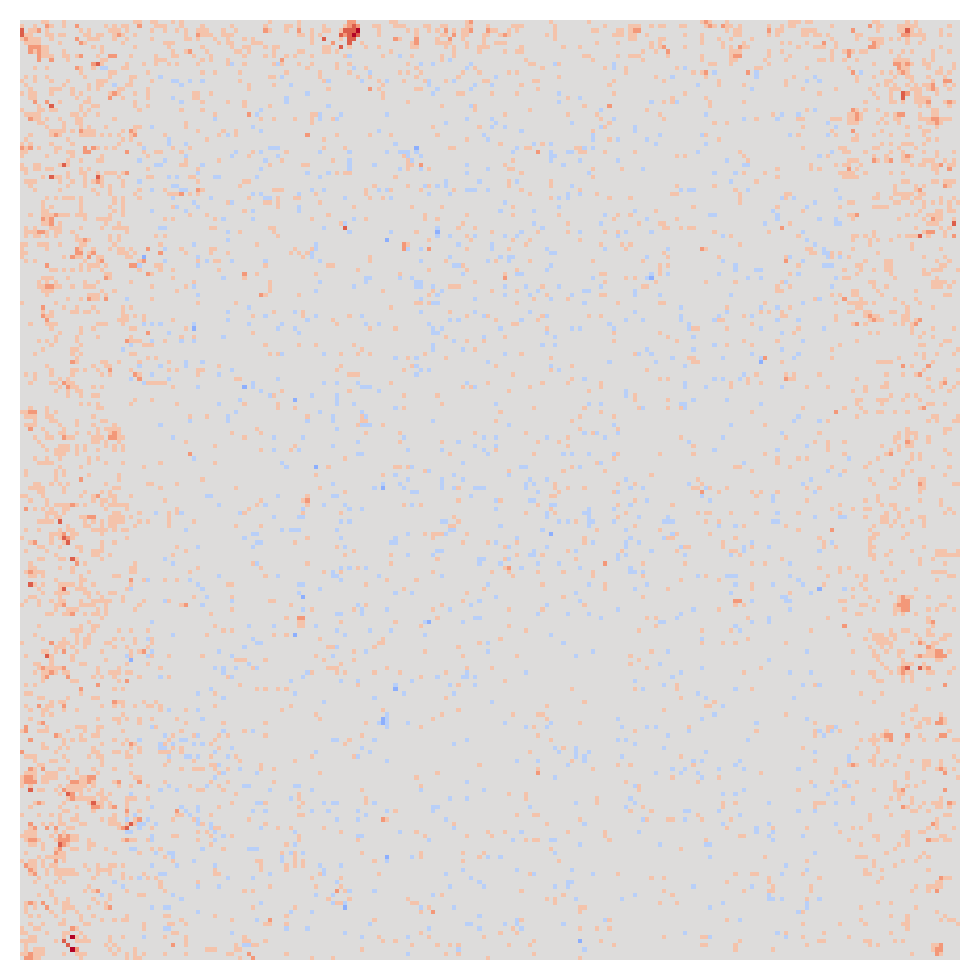
\includegraphics[height=1\linewidth]{01-images/05-resultate/uap_resnet/uap0-resnet18-mri-n200-robustificationslevel7.png}
        \caption{UAP 1 nach der Robustifikation}
    \end{subfigure}
    \hfill%
    \begin{subfigure}{0.19\linewidth}
        \centering
        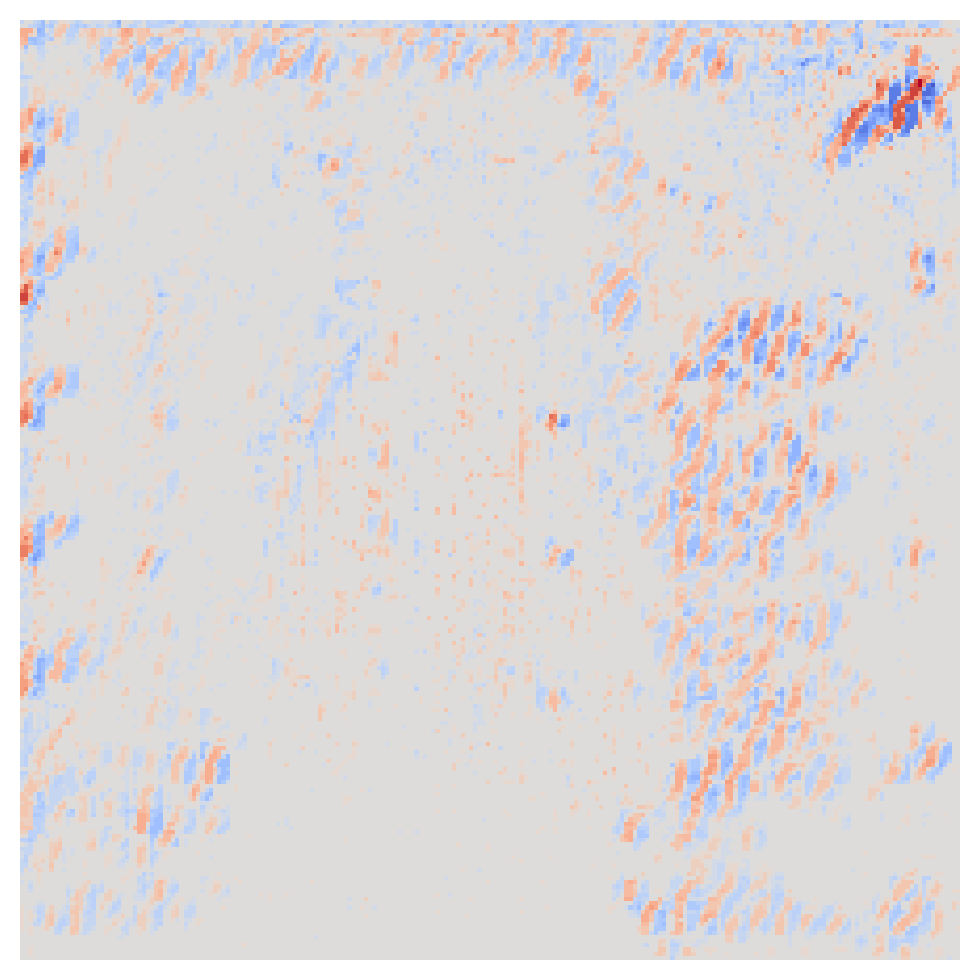
\includegraphics[height=1\linewidth]{01-images/05-resultate/uap_resnet/uap0-resnet18-covid-n200-robustificationslevel0.png}
        \caption{UAP 1 vor der Robustifikation}
    \end{subfigure}
    \begin{subfigure}{0.19\linewidth}
        \centering
        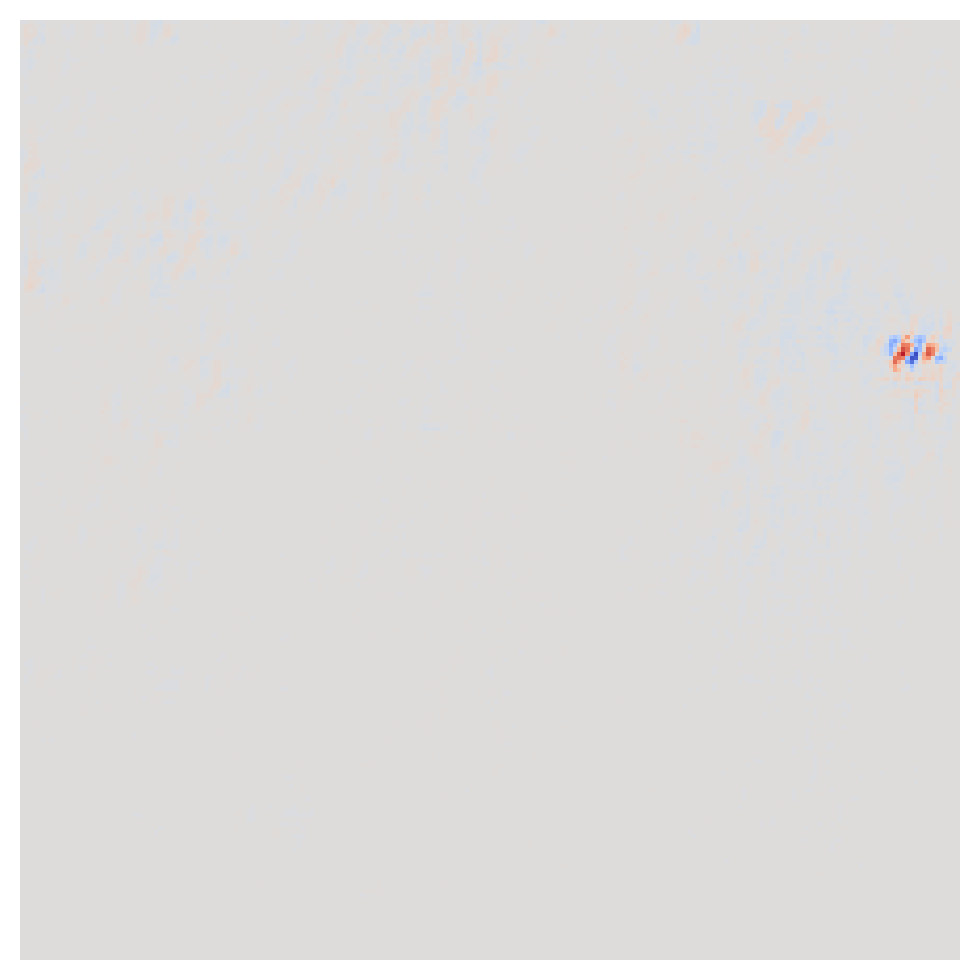
\includegraphics[height=1\linewidth]{01-images/05-resultate/uap_resnet/uap0-resnet18-covid-n200-robustificationslevel7.png}
        \caption{UAP 1 nach der Robustifikation}
    \end{subfigure}
    \caption{Generierte UAP vor und nach der Robustifikation für Covid und Hirntumor Datensatz}
    \label{fig:uap-resnet18-mri-rob0}
\end{figure}

Ein Vergleich von vor und nach der robustifikation ist in Abbildung \ref{} zu sehen

% UAP Robustifikationslevel
\begin{figure}[ht!]
    \centering
    \begin{subfigure}{0.095\linewidth}
        \centering
        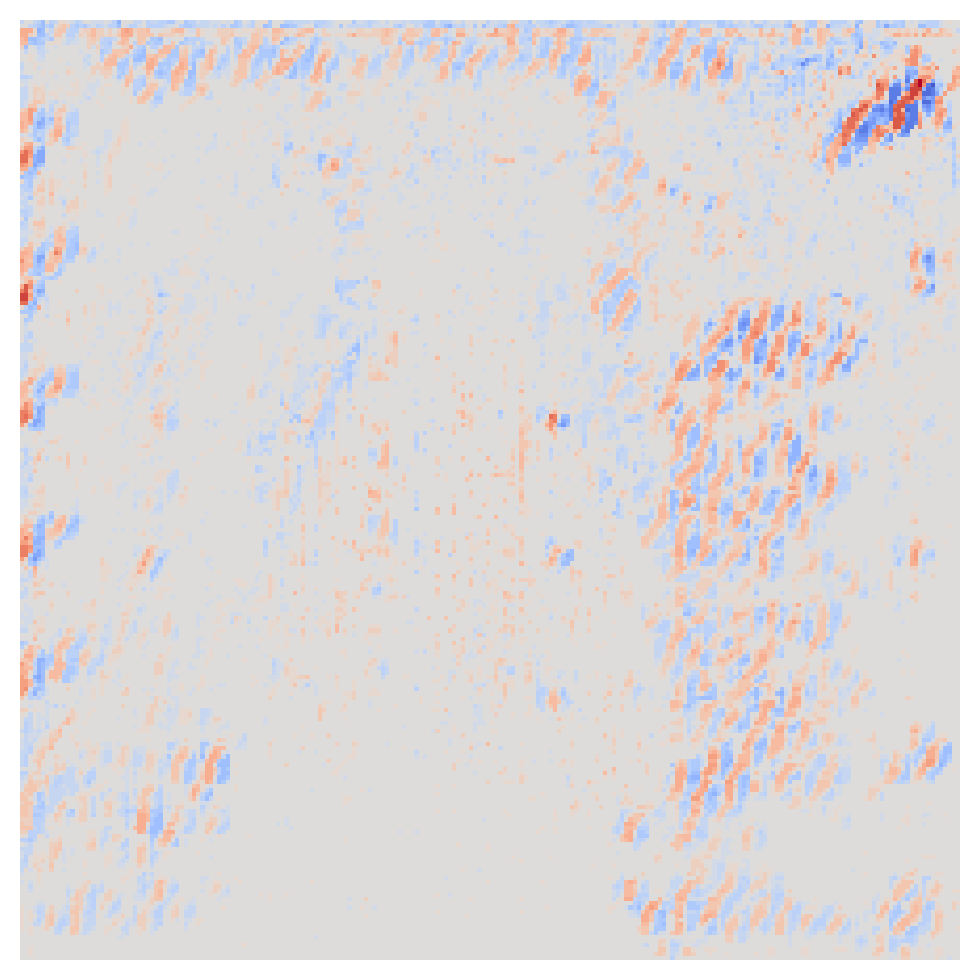
\includegraphics[height=1\linewidth]{01-images/05-resultate/uap_resnet/uap0-resnet18-covid-n200-robustificationslevel0.png}
        \caption{0}
    \end{subfigure}\hfill%
    \begin{subfigure}{0.095\linewidth}
        \centering
        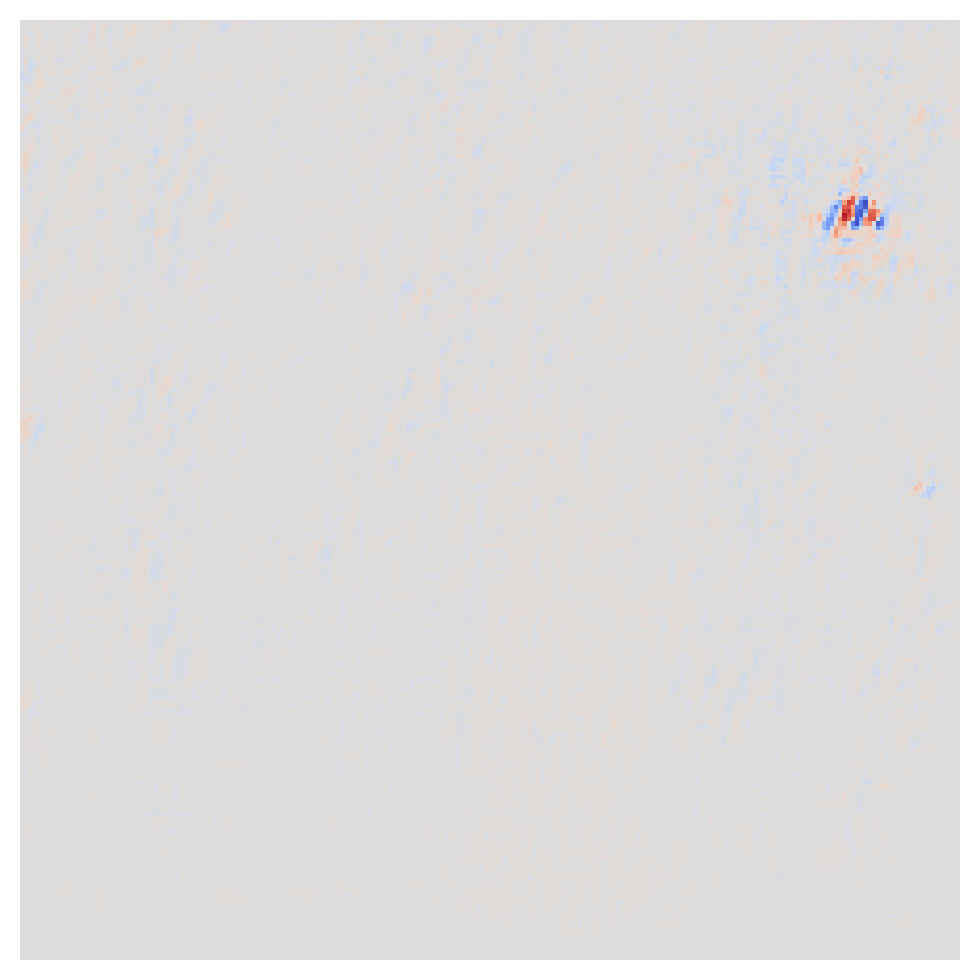
\includegraphics[height=1\linewidth]{01-images/05-resultate/uap_resnet/uap0-resnet18-covid-n200-robustificationslevel1.png}
        \caption{1}
    \end{subfigure}\hfill%
    \begin{subfigure}{0.095\linewidth}
        \centering
        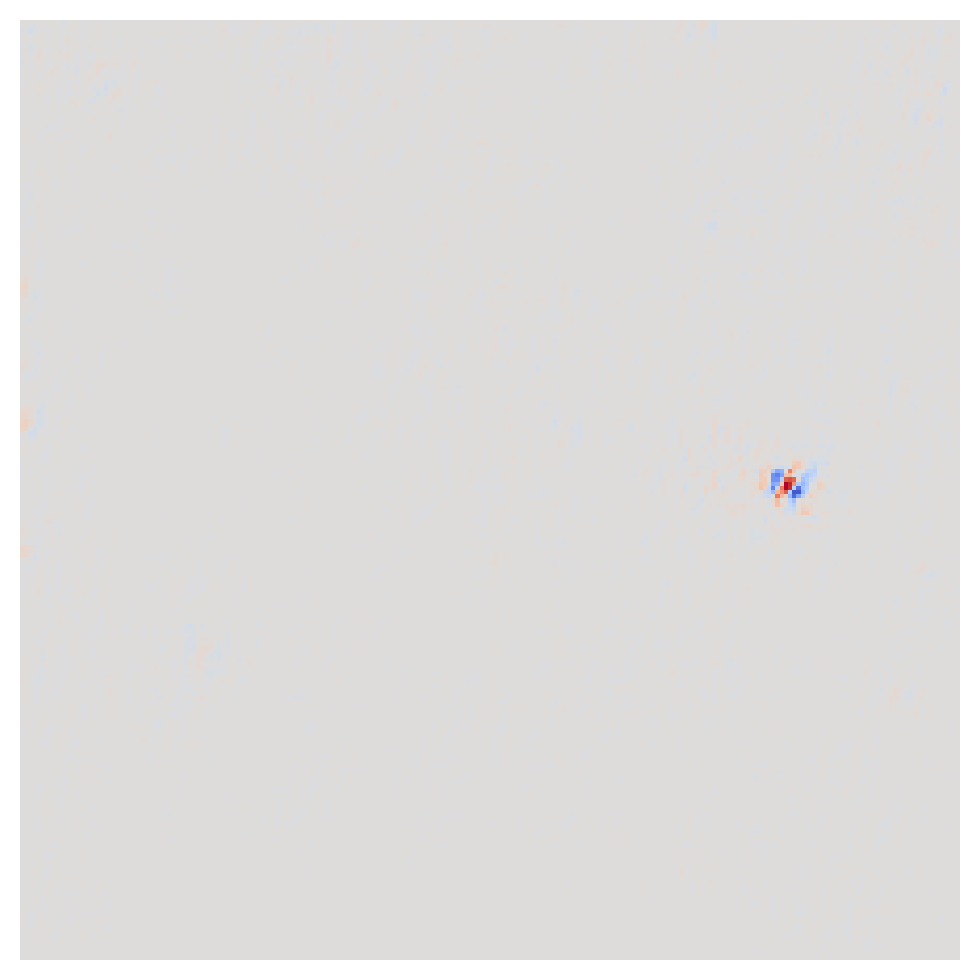
\includegraphics[height=1\linewidth]{01-images/05-resultate/uap_resnet/uap0-resnet18-covid-n200-robustificationslevel2.png}
        \caption{2}
    \end{subfigure}\hfill%
    \begin{subfigure}{0.095\linewidth}
        \centering
        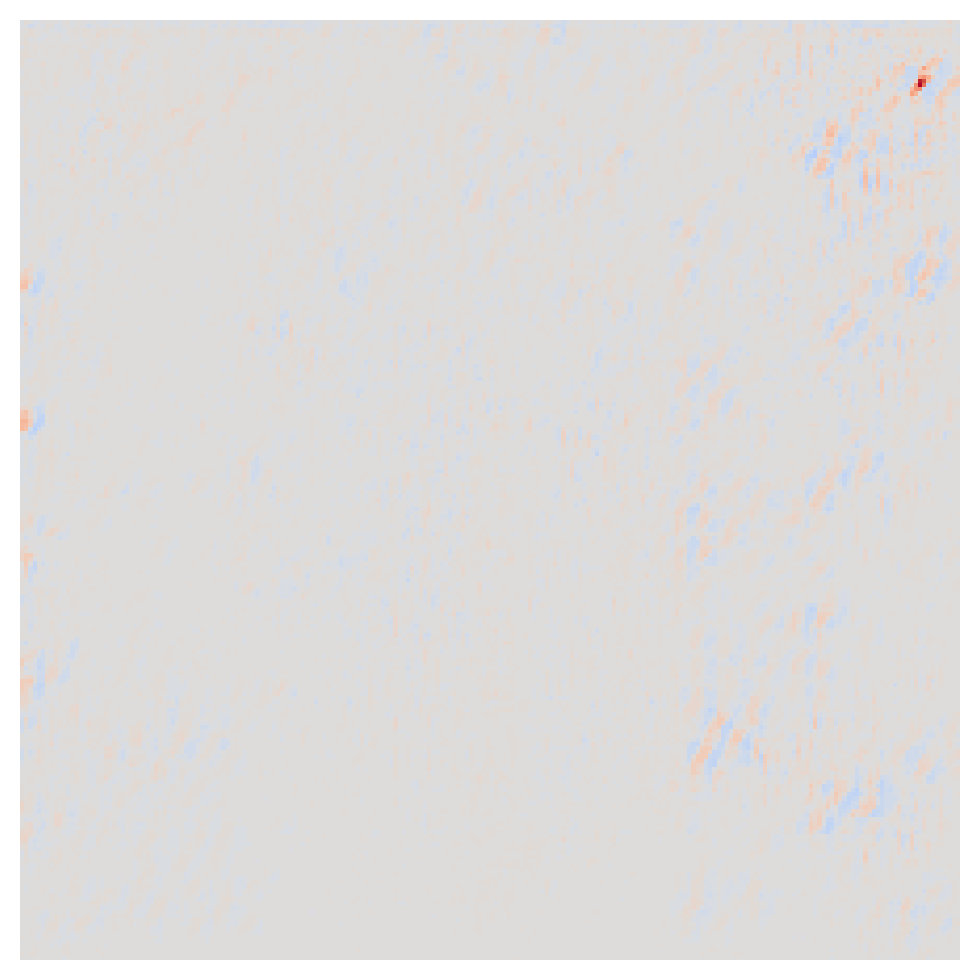
\includegraphics[height=1\linewidth]{01-images/05-resultate/uap_resnet/uap0-resnet18-covid-n200-robustificationslevel3.png}
        \caption{3}
    \end{subfigure}\hfill%
    \begin{subfigure}{0.095\linewidth}
        \centering
        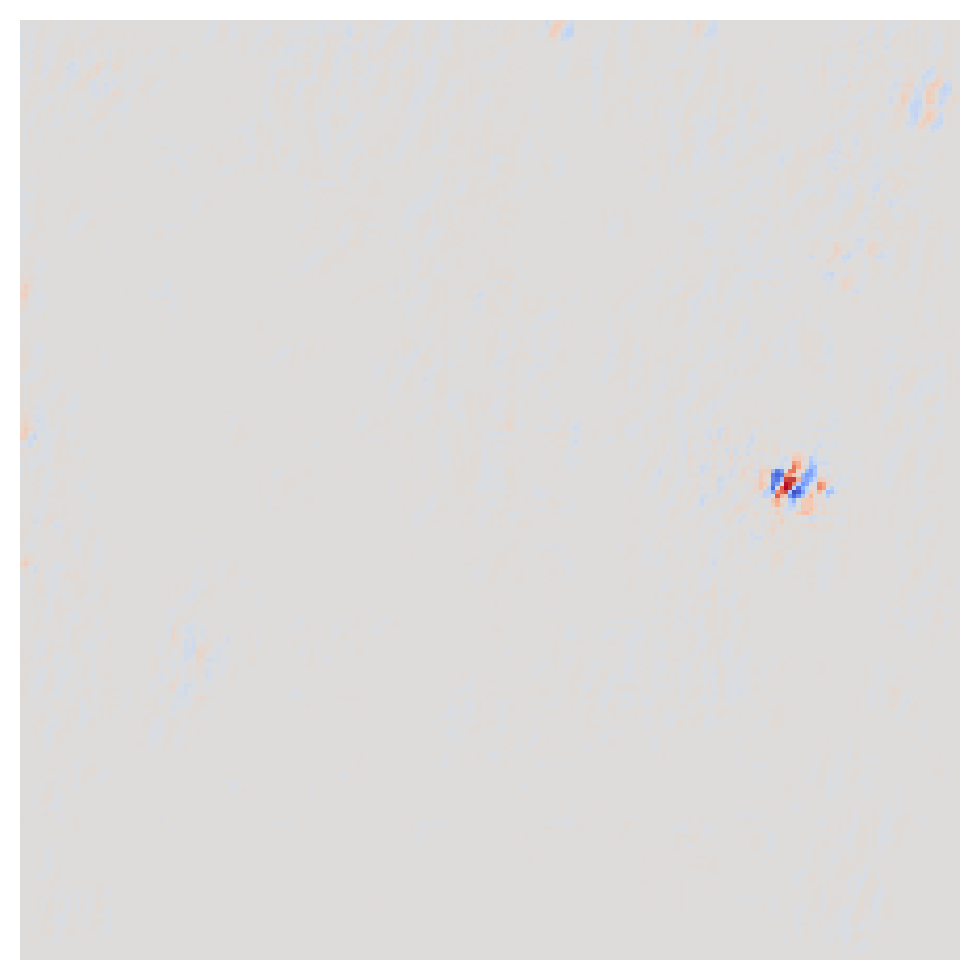
\includegraphics[height=1\linewidth]{01-images/05-resultate/uap_resnet/uap0-resnet18-covid-n200-robustificationslevel4.png}
        \caption{4}
    \end{subfigure}\hfill%
    \begin{subfigure}{0.095\linewidth}
        \centering
        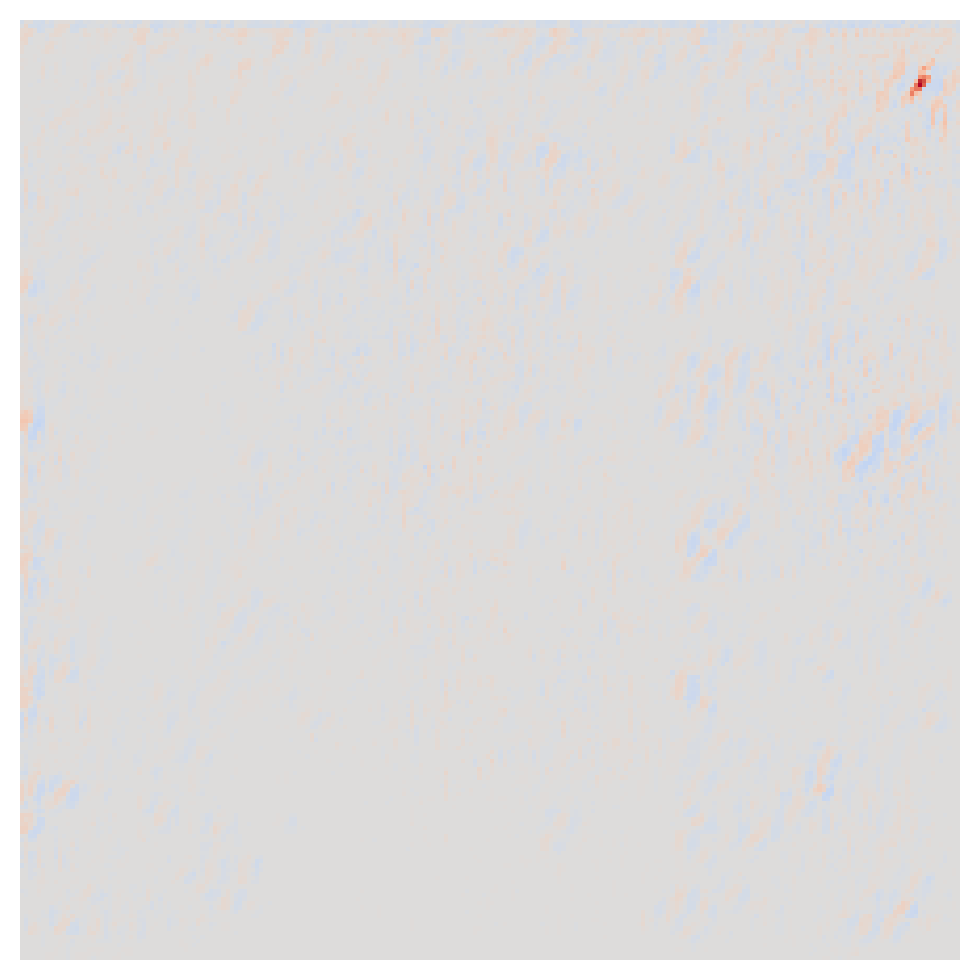
\includegraphics[height=1\linewidth]{01-images/05-resultate/uap_resnet/uap0-resnet18-covid-n200-robustificationslevel5.png}
        \caption{5}
    \end{subfigure}\hfill%
    \begin{subfigure}{0.095\linewidth}
        \centering
        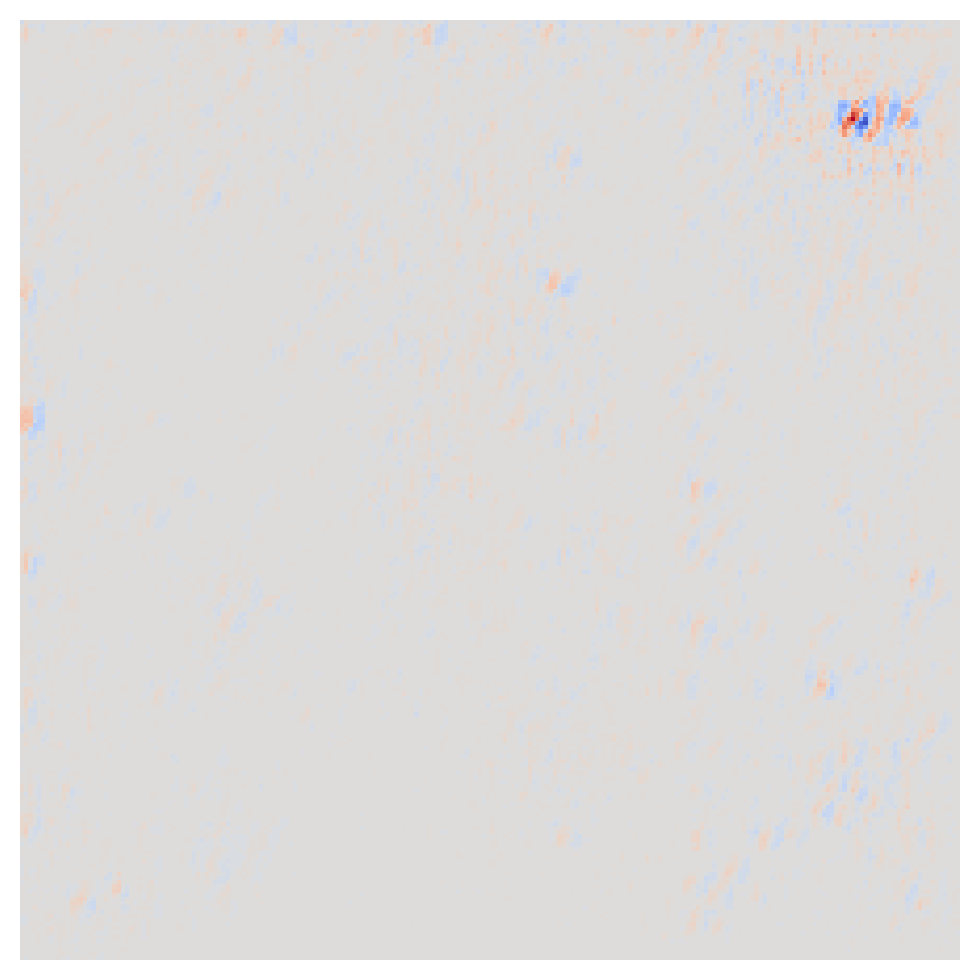
\includegraphics[height=1\linewidth]{01-images/05-resultate/uap_resnet/uap0-resnet18-covid-n200-robustificationslevel6.png}
        \caption{6}
    \end{subfigure}\hfill%
    \begin{subfigure}{0.095\linewidth}
        \centering
        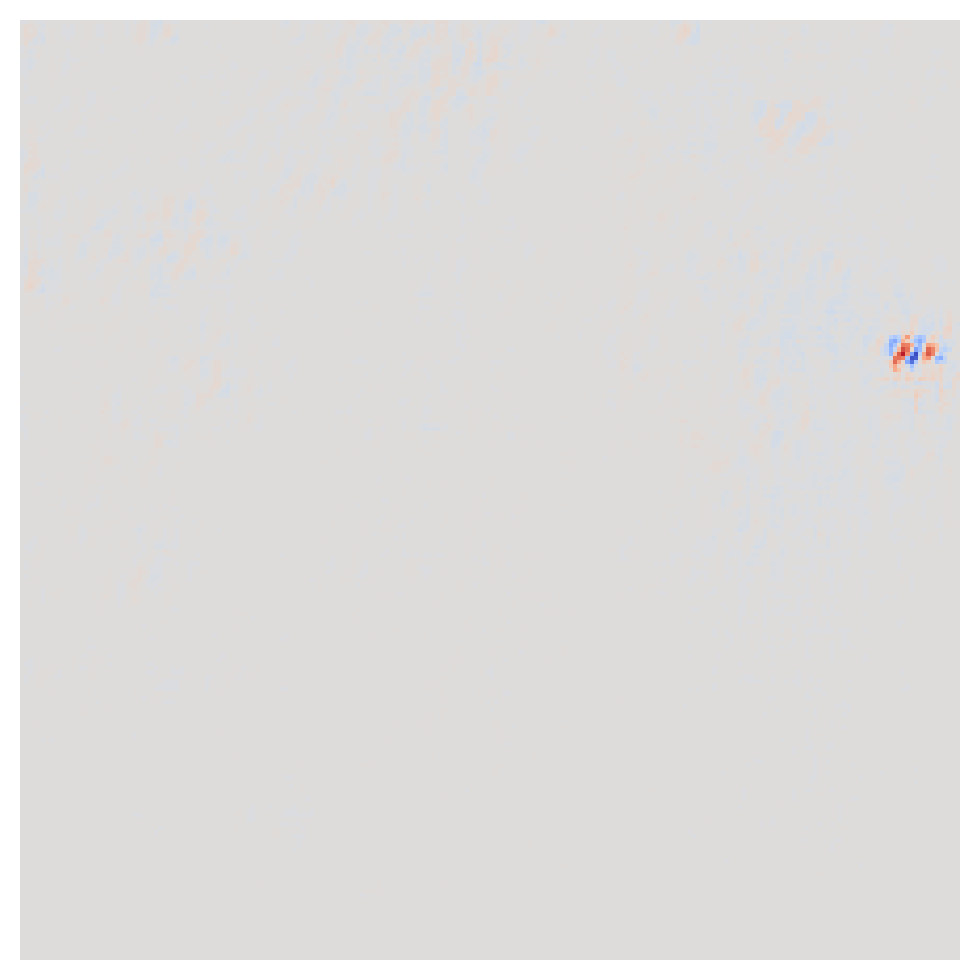
\includegraphics[height=1\linewidth]{01-images/05-resultate/uap_resnet/uap0-resnet18-covid-n200-robustificationslevel7.png}
        \caption{7}
    \end{subfigure}\hfill%
    \begin{subfigure}{0.095\linewidth}
        \centering
        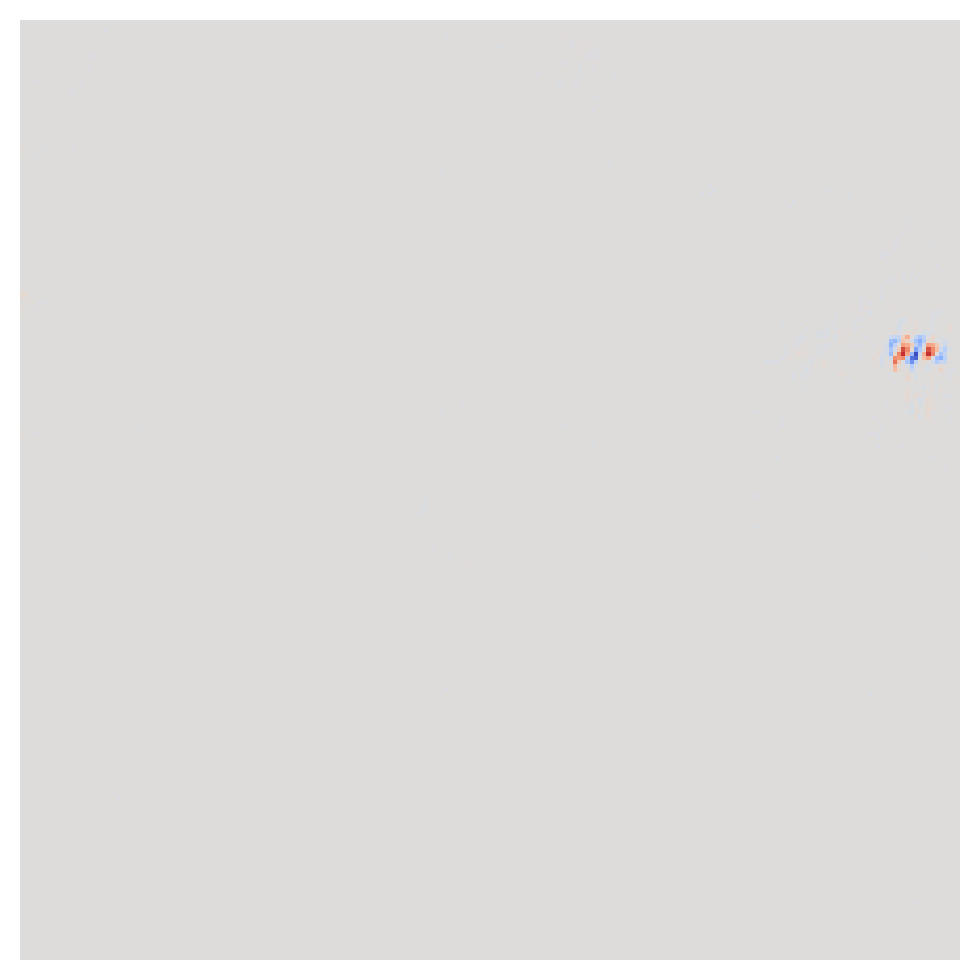
\includegraphics[height=1\linewidth]{01-images/05-resultate/uap_resnet/uap0-resnet18-covid-n200-robustificationslevel8.png}
        \caption{8}
    \end{subfigure}\hfill%
    \begin{subfigure}{0.095\linewidth}
        \centering
        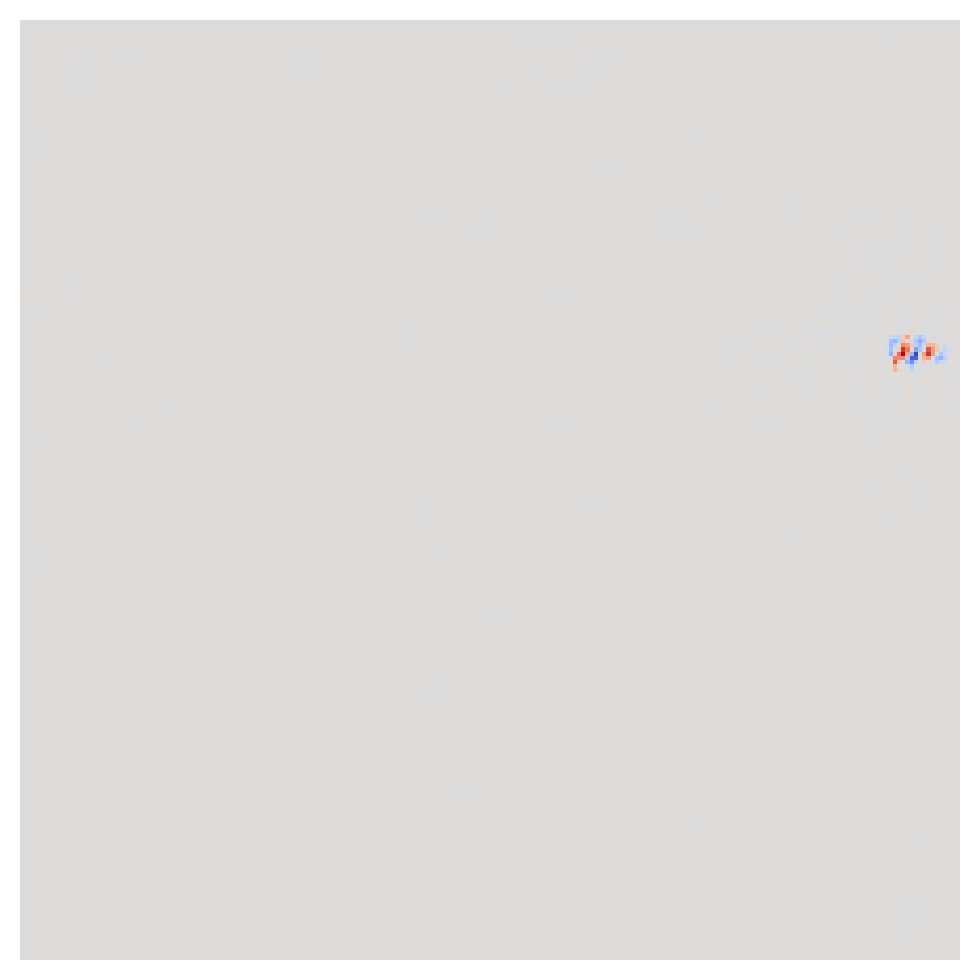
\includegraphics[height=1\linewidth]{01-images/05-resultate/uap_resnet/uap0-resnet18-covid-n200-robustificationslevel9.png}
        \caption{9}
    \end{subfigure}
    \caption{Generierte UAPs durch 200 Trainigsbilder des mit ResNet18 trainierten Hirntumor Datensatzes nach jeder Robustifikationslevel druch adversarial Training von links nach rechts}
    \label{fig:uap-resnet18-covidx-rob0}
\end{figure}

Hier in dieser Abbildung \ref{} sind jeweils nur die UAP Index 0 zu erkennen durch unterschiedliche Robustifikationslevel zu erkennen. 

\begin{figure}[ht!]
    \centering
    \begin{subfigure}{0.095\linewidth}
        \centering
        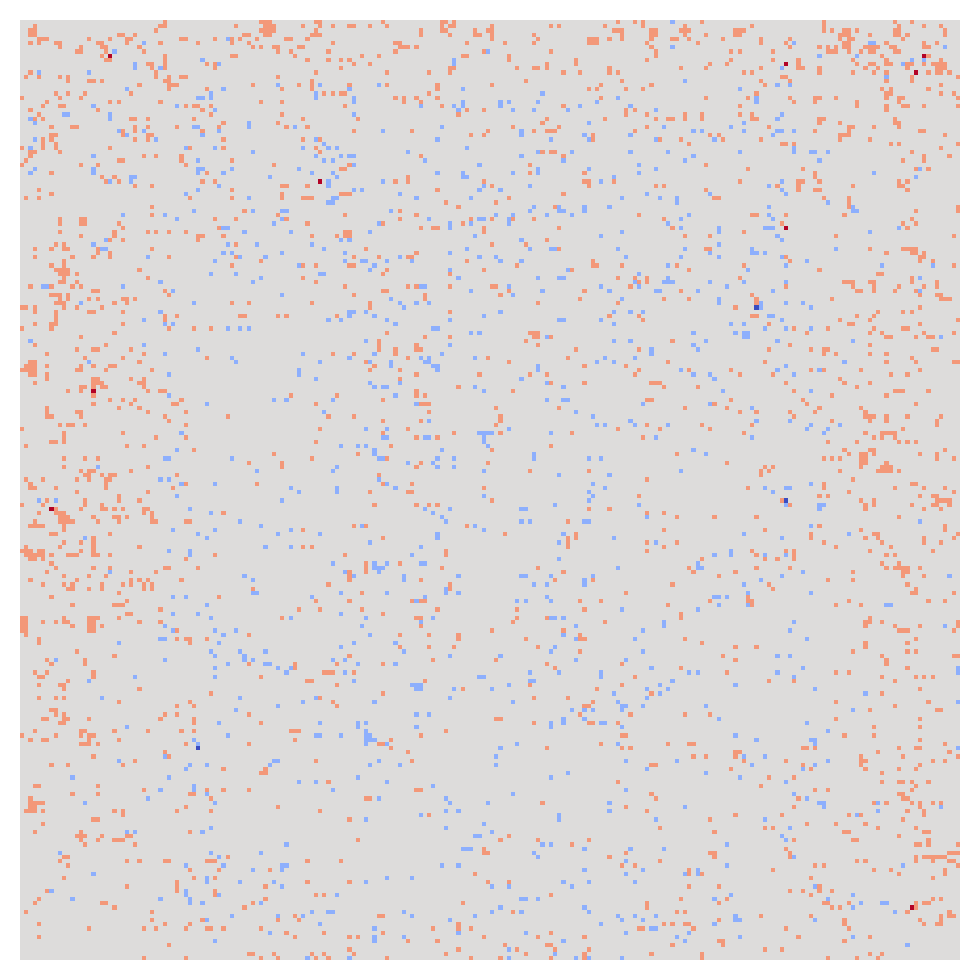
\includegraphics[height=1\linewidth]{01-images/05-resultate/uap_resnet/uap0-resnet18-mri-n200-robustificationslevel0.png}
        \caption{0}
    \end{subfigure}\hfill%
    \begin{subfigure}{0.095\linewidth}
        \centering
        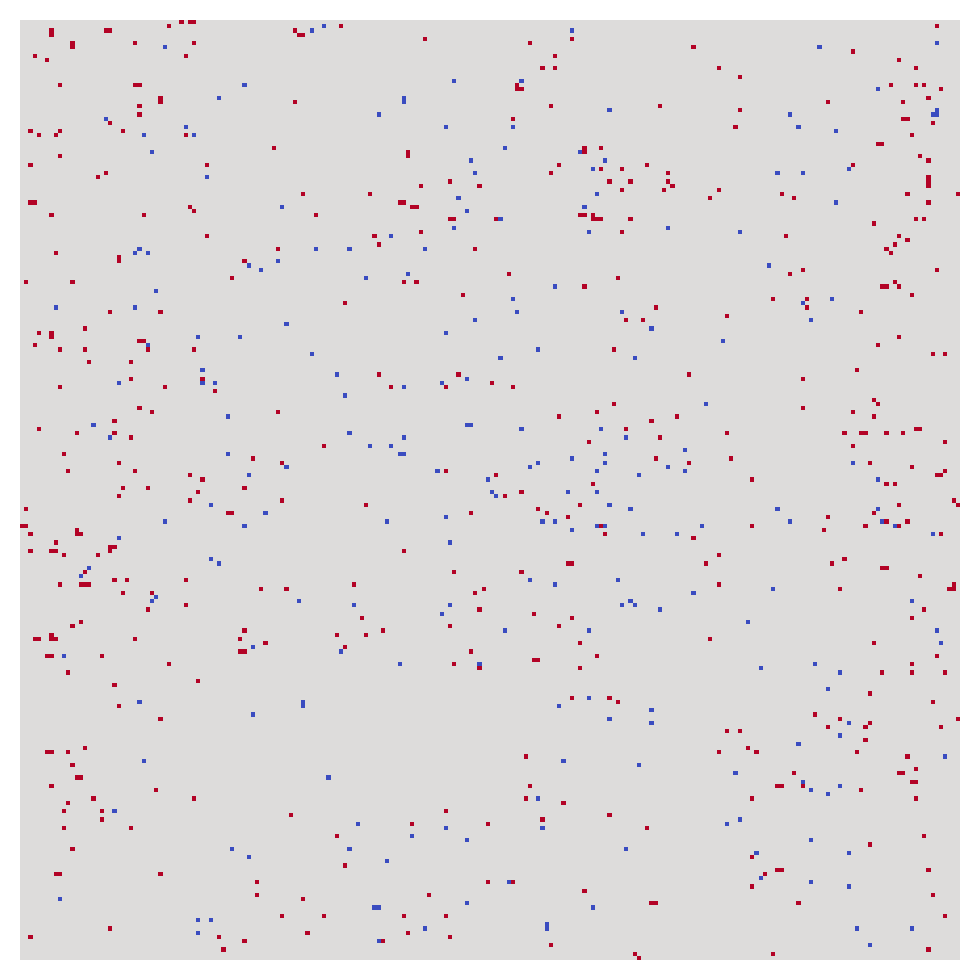
\includegraphics[height=1\linewidth]{01-images/05-resultate/uap_resnet/uap0-resnet18-mri-n200-robustificationslevel1.png}
        \caption{1}
    \end{subfigure}\hfill%
    \begin{subfigure}{0.095\linewidth}
        \centering
        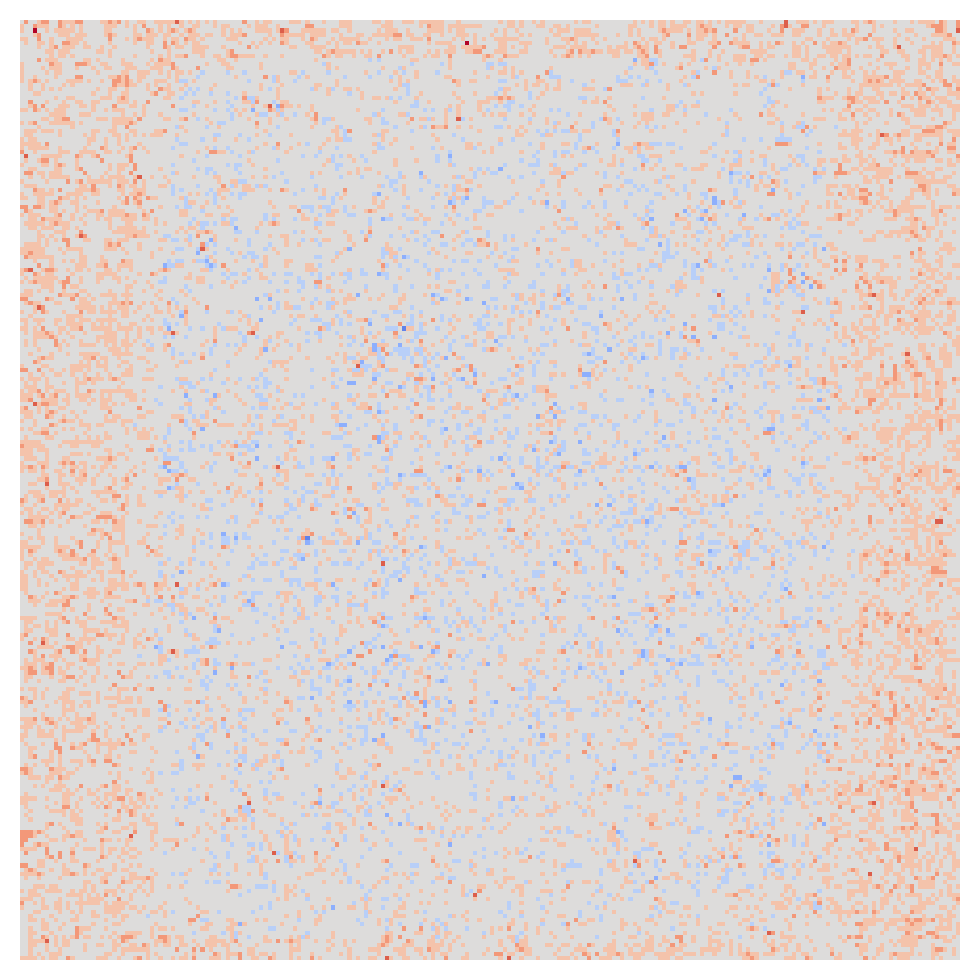
\includegraphics[height=1\linewidth]{01-images/05-resultate/uap_resnet/uap0-resnet18-mri-n200-robustificationslevel2.png}
        \caption{2}
    \end{subfigure}\hfill%
    \begin{subfigure}{0.095\linewidth}
        \centering
        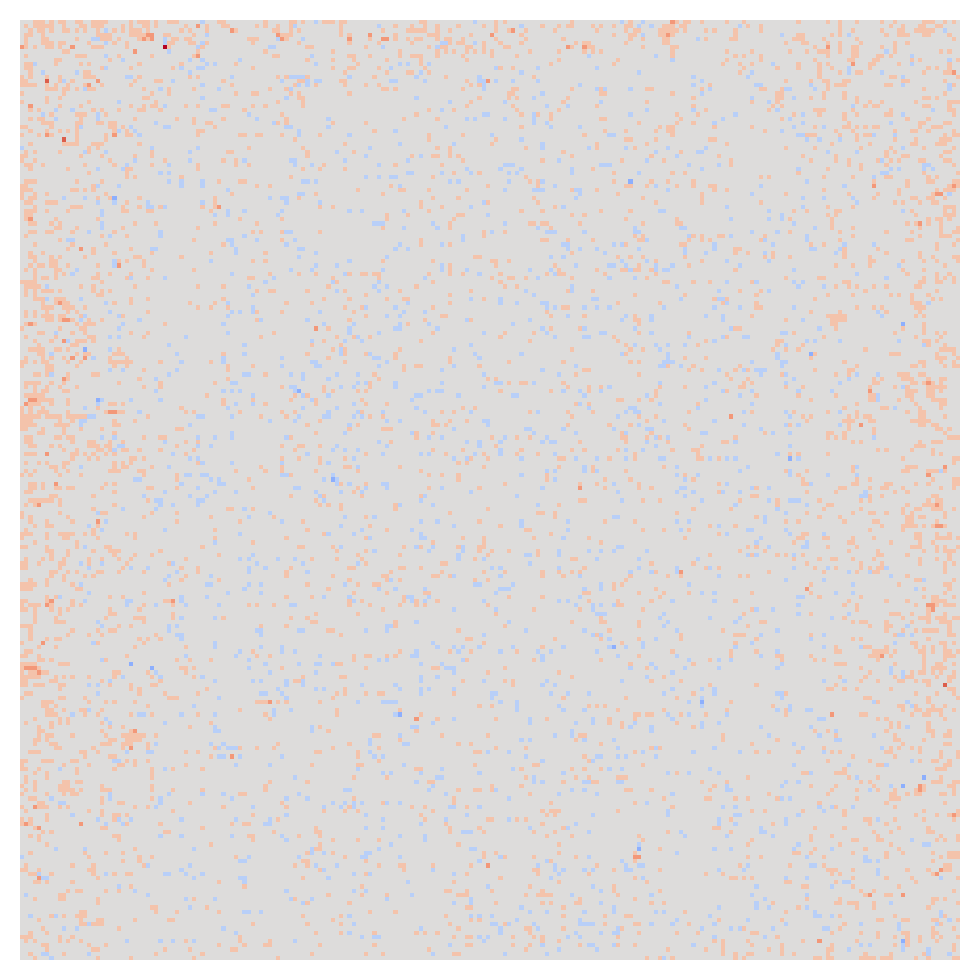
\includegraphics[height=1\linewidth]{01-images/05-resultate/uap_resnet/uap0-resnet18-mri-n200-robustificationslevel3.png}
        \caption{3}
    \end{subfigure}\hfill%
    \begin{subfigure}{0.095\linewidth}
        \centering
        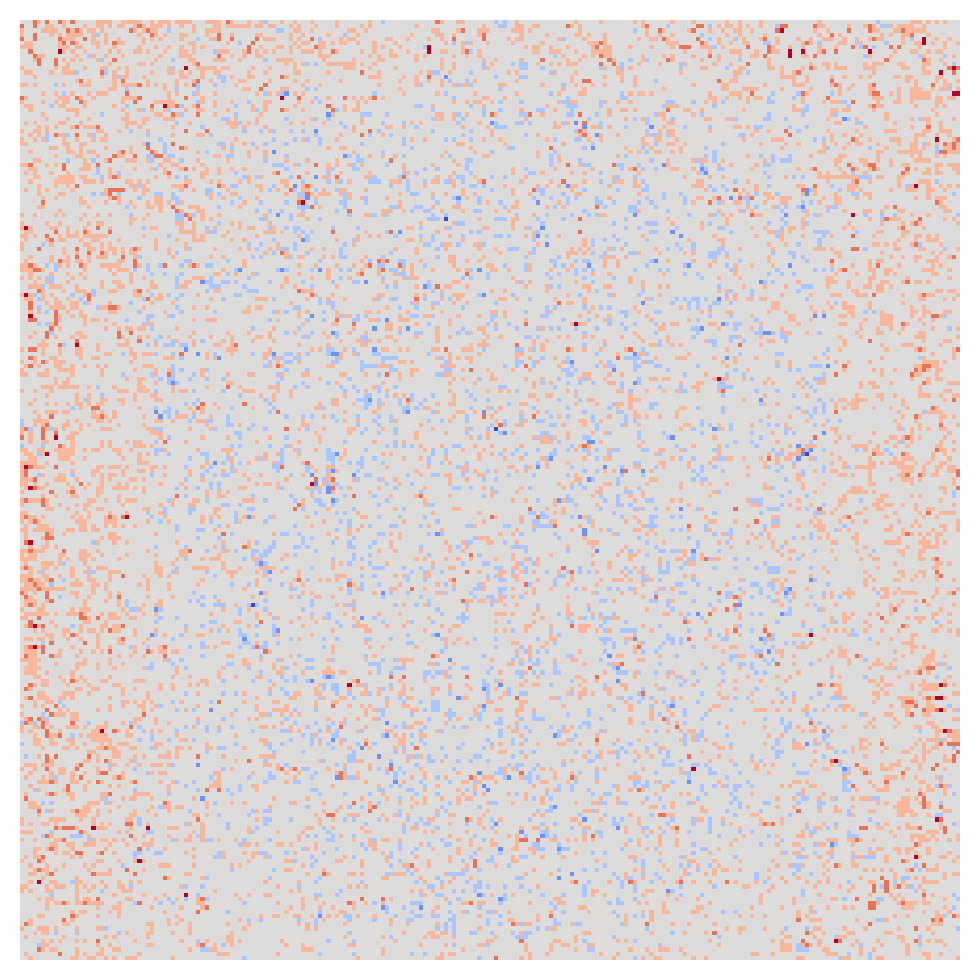
\includegraphics[height=1\linewidth]{01-images/05-resultate/uap_resnet/uap0-resnet18-mri-n200-robustificationslevel4.png}
        \caption{4}
    \end{subfigure}\hfill%
    \begin{subfigure}{0.095\linewidth}
        \centering
        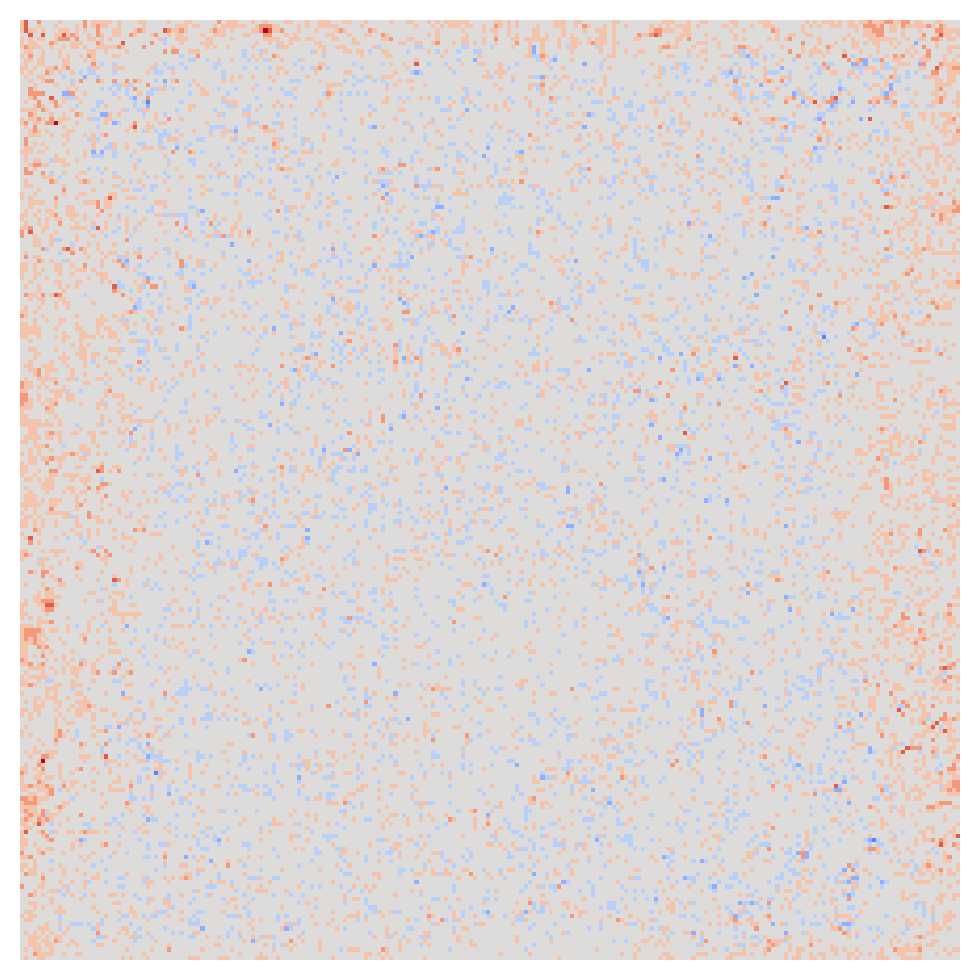
\includegraphics[height=1\linewidth]{01-images/05-resultate/uap_resnet/uap0-resnet18-mri-n200-robustificationslevel5.png}
        \caption{5}
    \end{subfigure}\hfill%
    \begin{subfigure}{0.095\linewidth}
        \centering
        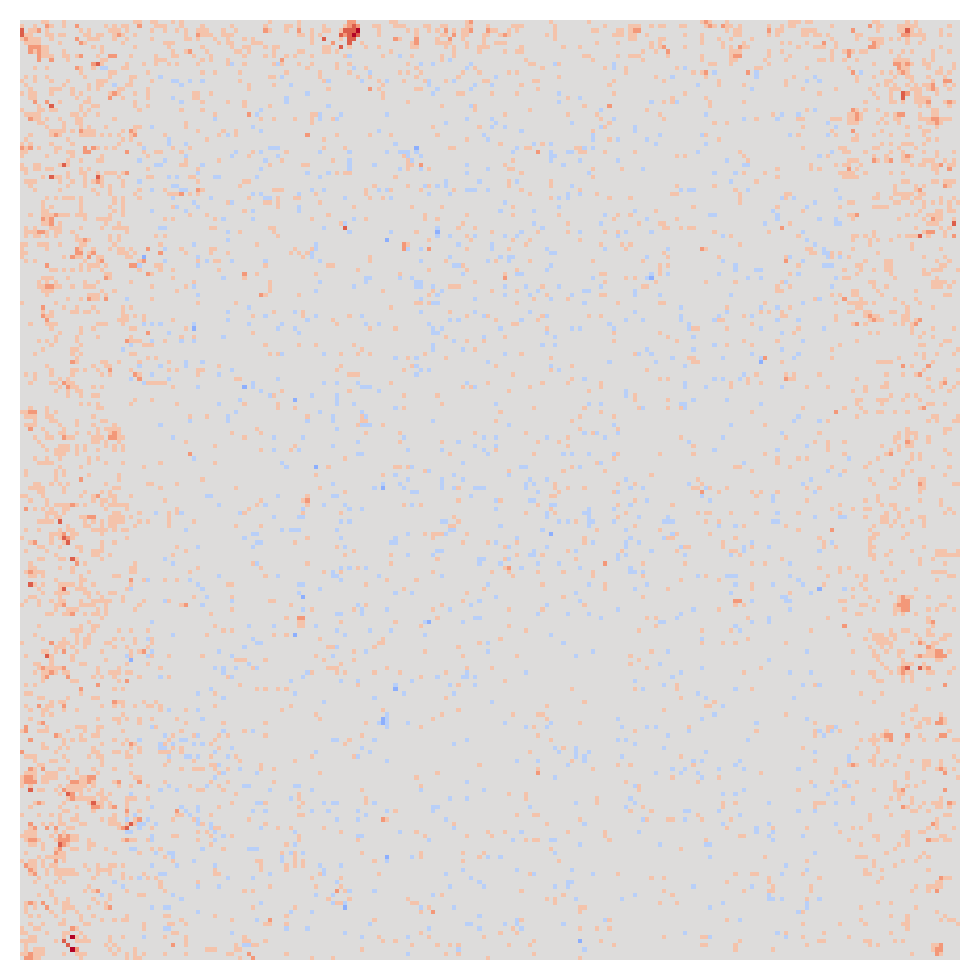
\includegraphics[height=1\linewidth]{01-images/05-resultate/uap_resnet/uap0-resnet18-mri-n200-robustificationslevel6.png}
        \caption{6}
    \end{subfigure}
    \caption{Generierte UAPs durch 200 Trainigsbilder des mit ResNet18 trainierten Hirntumor Datensatzes nach jeder Robustifikationslevel druch adversarial Training von links nach rechts}
    \label{fig:uap-resnet18-covidx-rob0}
\end{figure}



